\section{Terminal ingredients}

\subsection*{(a)}
$\mathcal{X}_{T}$ must be a positive invariant set (for the autonomous system $x_{t+1} = Ax_t$) and $P \succ 0$ a symmetric, positive definite matrix.

\subsection*{(b)}
If $\mathcal{X}_{T}$ is a positive invariant set, then $x \in \mathcal{X}_{T}$ and $Ax \in \mathcal{X}_{T}$.

Starting from $A^{\top}WA - W \preceq 0$:
\begin{align*}
x^{\top}(A^{\top}WA - W)x \leq 0 \\
(Ax)^{\top}WAx - x^{\top}Wx \leq 0 \\
\end{align*}
Since $x^{\top}Wx \leq 1$:
\[
(Ax)^{\top}WAx \leq x^{\top}Wx \leq 1 \\
\]
So $Ax_T \in \mathcal{X}_T$

For $I - r^2_xW \preceq 0$:
\begin{align*}
x^{\top}(I - r^2_xW)x \leq 0 \\
x^{\top}x - x^{\top}r^2_xWx \leq 0 \\
x^{\top}x \leq x^{\top}r^2_xWx \\
x^{\top}x/r^2_x \leq x^{\top}Wx \leq 1 \\
x^{\top}x \leq r^2_x
\end{align*}

Which already complies with $x^{\top}x \leq \| x \|^2_2 \leq r^2_x$

\subsection*{(c)}

\textbf{First Constraint}

Using the first hint
\begin{align*}
    A^{\top}M^{-1}A - M^{-1} \preceq 0 \\
    M(A^{\top}M^{-1}A)M - MM^{-1}M \preceq 0 \\
    MA^{\top}M^{-1}AM - M \succeq 0 \\
\end{align*}

Using Schur's complement lemma, the constraint is rewritten as:
\[
\left[
\begin{matrix}
    M & AM \\
    MA^{T} & M
\end{matrix}
\right]
\succeq 0
\]

\textbf{Second Constraint}
\begin{align*}
    I - r_x^2M^{-1} &\preceq 0 \\
    r_x^{-2}I &\preceq M^{-1} \\
\end{align*}
Using second hint
\begin{align*}
    r_x^2I &\succeq M \\
    r_x^2I - M &\succeq 0 \\
\end{align*}

\subsection*{(d)}
\begin{verbatim*}
W=
[[0.041 0.013]
 [0.013 0.198]]
\end{verbatim*}

\begin{figure}[H]
    \centering
    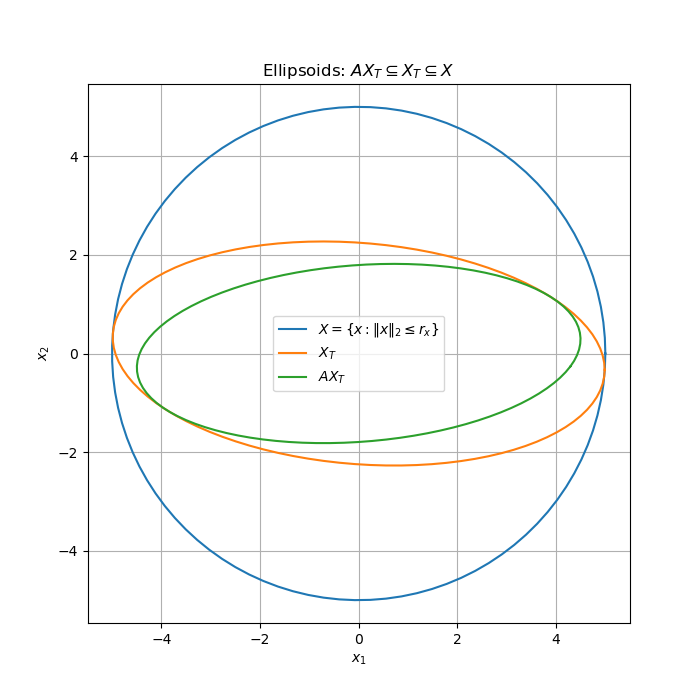
\includegraphics[width=0.5\textwidth]{figures/ellipsoids.png}
\end{figure}

\subsubsection*{(d)}

\begin{figure}[H]
    \centering
    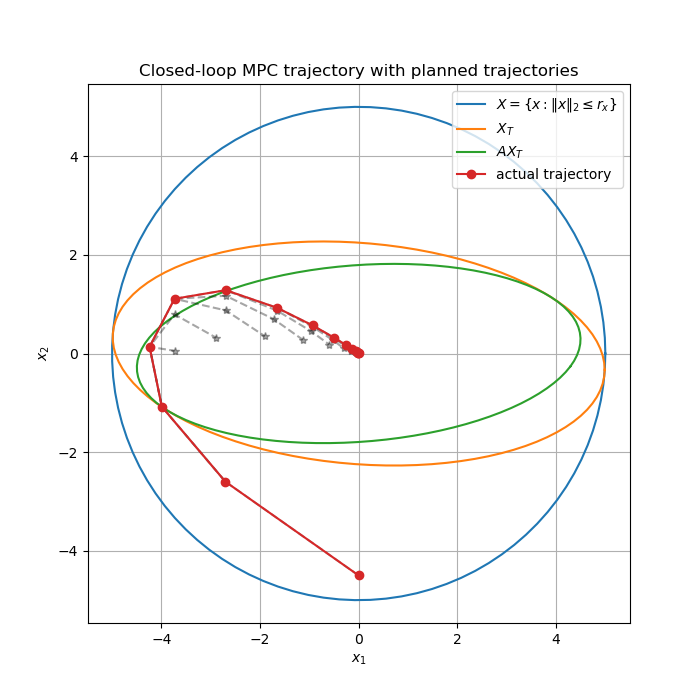
\includegraphics[width=0.5\textwidth]{figures/terminal_mpc_trajectory.png}
    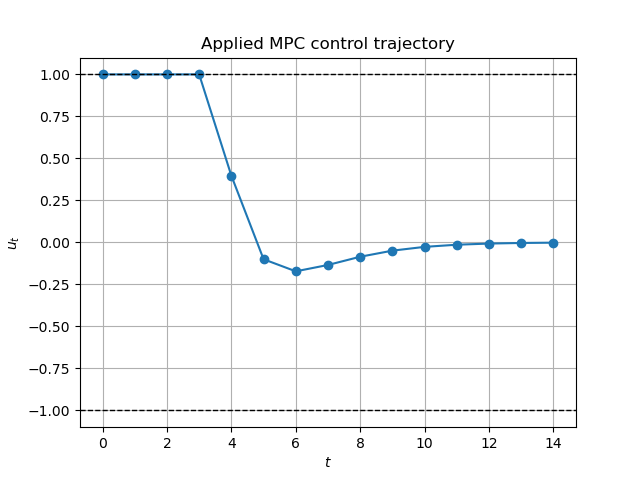
\includegraphics[width=0.5\textwidth]{figures/terminal_mpc_control.png}
\end{figure}

\subsection*{Code}
Code in \hyperref[terminal_ingredients]{Appendix}.
